\documentclass{beamer}

\mode<presentation> {

%\usetheme{default}
%\usetheme{AnnArbor}
%\usetheme{Antibes}
%\usetheme{Bergen}
%\usetheme{Berkeley}
%\usetheme{Berlin}
%\usetheme{Boadilla}
%\usetheme{CambridgeUS}
%\usetheme{Copenhagen}
%\usetheme{Darmstadt}
%\usetheme{Dresden}
%\usetheme{Frankfurt}
%\usetheme{Goettingen}
%\usetheme{Hannover}
%\usetheme{Ilmenau}
%\usetheme{JuanLesPins}
%\usetheme{Luebeck}
\usetheme{Madrid}
%\usetheme{Malmoe}
%\usetheme{Marburg}
%\usetheme{Montpellier}
%\usetheme{PaloAlto}
%\usetheme{Pittsburgh}
%\usetheme{Rochester}
%\usetheme{Singapore}
%\usetheme{Szeged}
%\usetheme{Warsaw}


%\usecolortheme{albatross}
%\usecolortheme{beaver}
%\usecolortheme{beetle}
%\usecolortheme{crane}
%\usecolortheme{dolphin}
%\usecolortheme{dove}
%\usecolortheme{fly}
%\usecolortheme{lily}
%\usecolortheme{orchid}
%\usecolortheme{rose}
%\usecolortheme{seagull}
%\usecolortheme{seahorse}
%\usecolortheme{whale}
%\usecolortheme{wolverine}

%\setbeamertemplate{footline} % To remove the footer line in all slides uncomment this line
%\setbeamertemplate{footline}[page number] % To replace the footer line in all slides with a simple slide count uncomment this line

%\setbeamertemplate{navigation symbols}{} % To remove the navigation symbols from the bottom of all slides uncomment this line
}

\usepackage{graphicx} % Allows including images
\usepackage{booktabs} % Allows the use of \toprule, \midrule and \bottomrule in tables
\usepackage{amsfonts}
\usepackage{mathrsfs}
\usepackage{amsmath,amssymb,graphicx}

%----------------------------------------------------------------------------------------
%	TITLE PAGE
%----------------------------------------------------------------------------------------

\title["9.2"]{9.2: Tests About a Population Mean}

\author{Taylor} 
\institute[UVA] 
{
University of Virginia \\
\medskip
\textit{} 
}
\date{} 

\begin{document}
%----------------------------------------------------------------------------------------

\begin{frame}
\titlepage 
\end{frame}
%----------------------------------------------------------------------------------------

\begin{frame}
\frametitle{Motivation}

We learned about how to do confidence intervals for three cases:
\begin{enumerate}
\item normal population with known variance
\item large-sample intervals
\item normal population with unknown variance.
\end{enumerate}

Now we'll learn how to test hypotheses pertaining to $\mu$ in these same three cases.
\end{frame}
%----------------------------------------------------------------------------------------


\begin{frame}
\frametitle{Case 1:}

 $X_1, \ldots, X_n \overset{iid}{\sim} \mathcal{N}(\mu, \sigma^2)$ (and we know $\sigma^2$). Then $\bar{X} \sim \mathcal{N}(\mu, \sigma^2/n)$.
\newline

Let's say we're testing $H_0: \mu = \mu_0$ versus $H_a: \mu > \mu_0$. So we assume $H_0$ is correct and see if we can ``break" it. Assuming it's true, then $\bar{X} \sim \mathcal{N}(\mu_0, \sigma^2/n)$. Since this is a ``right-tailed" test, we reject $H_0$ if we observe big $\bar{X}$. 
\newline


\end{frame}
%----------------------------------------------------------------------------------------


\begin{frame}
\frametitle{Case 1:}

Let $N_{\alpha}$ be the $(1-\alpha)$th percentile associated with the $\mathcal{N}(\mu_0, \sigma^2/n)$ distribution. 

\[
\bar{X} > N_{\alpha} \iff \frac{\bar{X} - \mu_0}{\frac{\sigma}{\sqrt{n}}} > z_{\alpha}
\]

So we reject when $\bar{X}$ is really big, or when $Z = \frac{\bar{X}-\mu_0}{\sigma/ \sqrt{n}}$ is really big. It's relative though, so we have different percentiles.
\end{frame}
%----------------------------------------------------------------------------------------


\begin{frame}
\frametitle{Case 1:}

a summary:

\begin{enumerate}
\item the null hypothesis is always $H_0: \mu = \mu_0$ for some specific $\mu_0$
\item our test statistic is $Z = \frac{\bar{X}-\mu_0}{\sigma/ \sqrt{n}}$
\item if $H_a: \mu > \mu_0$, then we reject if $Z > z_{\alpha}$
\item if $H_a: \mu < \mu_0$, then we reject if $Z < -z_{\alpha}$
\item if $H_a: \mu \neq \mu_0$, then we reject if $Z > z_{\alpha/2}$ OR if $Z < -z_{\alpha/2}$
\end{enumerate}


\end{frame}
%----------------------------------------------------------------------------------------


\begin{frame}
\frametitle{Example 9.6 in the book}

``A manufacturer of sprinkler systems used for fire protection in office buildings claims that the true average system-activation temperature is 130 degrees. A sample of $n=9$ systems, when tested, yields a sample average activation temperature of 131.08 degrees. If the distribution of activation times is normal with standard deviation 1.5 degrees, does the data contradict the manufacturer's claim at significance level $\alpha = .01$?

\end{frame}
%----------------------------------------------------------------------------------------

\begin{frame}
\frametitle{Example 9.6 in the book}

\begin{enumerate}
\item $H_0: \mu = 130$ \pause
\item $H_a: \mu \neq 130$ \pause
\item $Z = \frac{\bar{X} - \mu_0}{\sigma / \sqrt{n}} = \frac{131.08 - 130}{1.5 / \sqrt{9}} = 2.16$
\item $z_{\alpha/2} = 2.575829$, $-z_{\alpha/2} = -2.575829$
\end{enumerate}

So we fail to reject at $\alpha = .01$ significance.

\end{frame}
%----------------------------------------------------------------------------------------


\begin{frame}
\frametitle{Side-Note}

The book mentions how we could get the same result by doing a 99\% confidence interval for $\mu$ and rejecting $H_0$ if this interval didn't contain 130. This follows from that math we did with confidence intervals; remember that
\[
\bar{X} - z_{\alpha/2}\frac{\sigma}{\sqrt{n}} \le \mu \le \bar{X} + z_{\alpha/2}\frac{\sigma}{\sqrt{n}}
\]
is the same event as 
\[
-z_{\alpha/2} \le \frac{\bar{X} - \mu}{\sigma / \sqrt{n}} \le z_{\alpha/2}
\]

So if we assume that $\mu = \mu_0$, we can see that our test statistic is in the rejection region if and only if our confidence interval does not cover $\mu_0$ (like it should). This can be seen by taking the complement event of the things above.
\end{frame}
%----------------------------------------------------------------------------------------

\begin{frame}
\frametitle{Type 2 Error Calculation}

Calculating type 2 error for these tests isn't that bad. Recall that this depends on what $\mu$ actually is. WLOG assume we're talking about a right-tail test (i.e. $H_a: \mu > \mu_0$).

\begin{align*}
\beta(\mu') &= P( \text{ not rejecting $H_0$ when } \mu = \mu')\\
&= P\left( \frac{\bar{X} - \mu_0}{\sigma/\sqrt{n}} \le z_{\alpha} \text{ when } \mu = \mu'\right) \\
&= P(\bar{X} \le \mu_0 + z_{\alpha}\frac{\sigma}{\sqrt{n}} \text{ when } \mu = \mu') \\
&= P\left( \frac{\bar{X} - \mu'}{\sigma/ \sqrt{n}} \le z_{\alpha} + \frac{\mu_0 - \mu'}{\sigma / \sqrt{n}} \text{ when } \mu = \mu' \right) \\
&= \Phi \left( z_{\alpha} + \frac{\mu_0 - \mu'}{\sigma / \sqrt{n}} \right)
\end{align*}


\end{frame}
%----------------------------------------------------------------------------------------
\begin{frame}
\frametitle{Type 2 Error Calculation}

So
\[
\beta(\mu') = \Phi \left( z_{\alpha} + \frac{\mu_0 - \mu'}{\sigma / \sqrt{n}} \right)
\]

The plot below assumes that $\mu_0 = 10$, $\sigma = 3$ and $n=100$ and $\alpha = .05$

\begin{center}
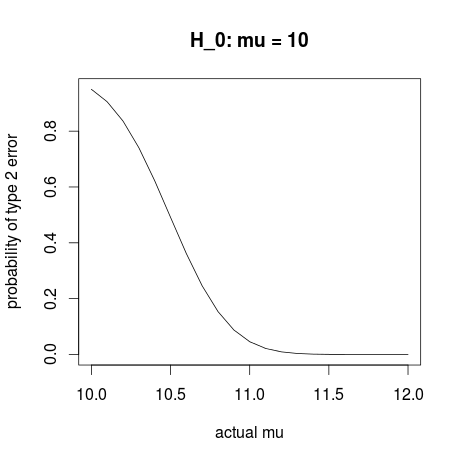
\includegraphics[width=55mm]{pics/type_2_error.png}
\end{center}

\end{frame}
%----------------------------------------------------------------------------------------


\begin{frame}
\frametitle{Case 2}

We don't know what distribution the data is coming from now, but we can assume that our data is really big. In chapter 8 we said 
\[
Z = \frac{\bar{X} - \mu}{S /\sqrt{n}} \overset{\text{approx.}}{\sim} \mathcal{N}(0,1).
\]
In this chapter, we use this again, but we further assume that $\mu = \mu_0$. In other words, we further assume that the null hypothesis is true. 
\[
Z = \frac{\bar{X} - \mu_0}{S /\sqrt{n}} \overset{\text{approx.}}{\sim} \mathcal{N}(0,1).
\]

\end{frame}
%----------------------------------------------------------------------------------------


\begin{frame}
\frametitle{Example 9.8 on page 442}

``A sample of bills for meals was obtained at a restaurant (by Erich Brandt). For each of 70 bills the tip was found as a percentage of the raw bill (before taxes). Does it appear that the population mean tip percentage for this restaurant exceeds the standard 15\%?"
\newline

Looking at the histogram on page 442, these data are definitely not normally distributed...
\end{frame}
%----------------------------------------------------------------------------------------


\begin{frame}
\frametitle{Example 9.8 on page 442}

...but $\bar{X}$ is (approximately):

\begin{enumerate}
\item $H_0: \mu = 15$
\item $H_a: \mu > 15$
\item $Z = \frac{\bar{X} - \mu_0}{S / \sqrt{n}} = \frac{17.99 - 15}{5.937 / \sqrt{70}} = 4.21$
\item $z_{\alpha} = z_{.05} = 1.645$
\end{enumerate}

So we reject $H_0$ at significance level $\alpha = .05$
\end{frame}
%----------------------------------------------------------------------------------------

\begin{frame}
\frametitle{Case 3}

Now we assume $X_1, \ldots, X_n \overset{iid}{\sim} \mathcal{N}(\mu, \sigma^2)$. But we don't know $\sigma^2$. 
\newline

Even if we don't know it, recall that 
\[
T = \frac{\bar{X} - \mu}{S/\sqrt{n}} \sim t_{n-1}
\]

so our new test statistic is $\frac{\bar{X} - \mu_0}{S/\sqrt{n}}$, and our percentiles depend on the degrees of freedom.

\end{frame}
%----------------------------------------------------------------------------------------


\begin{frame}
\frametitle{Case 3}

a summary:
\begin{enumerate}
\item $H_0: \mu = \mu_0$
\item test statistic: $T = \frac{\bar{X} - \mu_0}{S/\sqrt{n}}$
\item if $H_a: \mu > \mu_0$, then we reject if $T > t_{\alpha,n-1}$
\item if $H_a: \mu < \mu_0$, then we reject if $T < -t_{\alpha,n-1}$
\item if $H_a: \mu \neq \mu_0$, then we reject if $T > t_{\alpha/2,n-1}$ OR if $T < -t_{\alpha/2,n-1}$
\end{enumerate}


\end{frame}
%----------------------------------------------------------------------------------------

\begin{frame}
\frametitle{Type 2 Error Calculation}


Calculating type 2 error for these tests is much more difficult. Let's just see why...

\begin{align*}
\beta(\mu') &= P( \text{ not rejecting $H_0$ when } \mu = \mu')\\
&= P(\bar{X} \le \mu_0 + t_{\alpha,n-1}\frac{S}{\sqrt{n}} \text{ when } \mu = \mu') \\
&= P\left( \frac{\bar{X} - \mu'}{S/ \sqrt{n}} \le t_{\alpha,n-1} + \frac{\mu_0 - \mu'}{S / \sqrt{n}} \text{ when } \mu = \mu' \right) 
\end{align*}

Last time we had $\Phi \left( z_{\alpha} + \frac{\mu_0 - \mu'}{\sigma / \sqrt{n}} \right)$. This was okay because it was the cdf at a point. But now we have the cdf evaluated at a \textbf{random} point...

\end{frame}
%----------------------------------------------------------------------------------------


\begin{frame}
\frametitle{Example 9.9 on page 444}

``A well-designed and safe workplace can contribute greatly to increased productivity. It is especially important that workers not be asked to perform tasks, such as lifting, that exceed their capabilities...Assuming that MAWL is normally distributed, does the following data suggest that the population mean MAWL exceeds 25?"
\pause
\newline

\begin{enumerate}
\item $H_0: \mu = 25$ \pause
\item $H_a: \mu > 25$ \pause
\item $T = \frac{\bar{X} - 25}{S/\sqrt{n}} = \frac{27.54 - 25}{5.47 / \sqrt{5}} = 1.04$ \pause
\item $t_{\alpha, n-1} = 2.132$ 
\end{enumerate}

so we do not reject $H_0$ at $\alpha = .05$ significance.

\end{frame}
%----------------------------------------------------------------------------------------




\end{document} 
